% Important: If latex complains about unicode characters,
% please use "\usepackage[utf8x]{inputenc}" in your preamble
% You can change the size of the picture by putting it into the construct:
% 1) \resizebox{10cm}{!}{"below picture"} to scale horizontally to 10 cm
% 2) \resizebox{!}{15cm}{"below picture"} to scale vertically to 15 cm
% 3) \resizebox{10cm}{15cm}{"below picture"} a combination of above two
% It is not recomended to use the scale option of the tikzpicture environment.
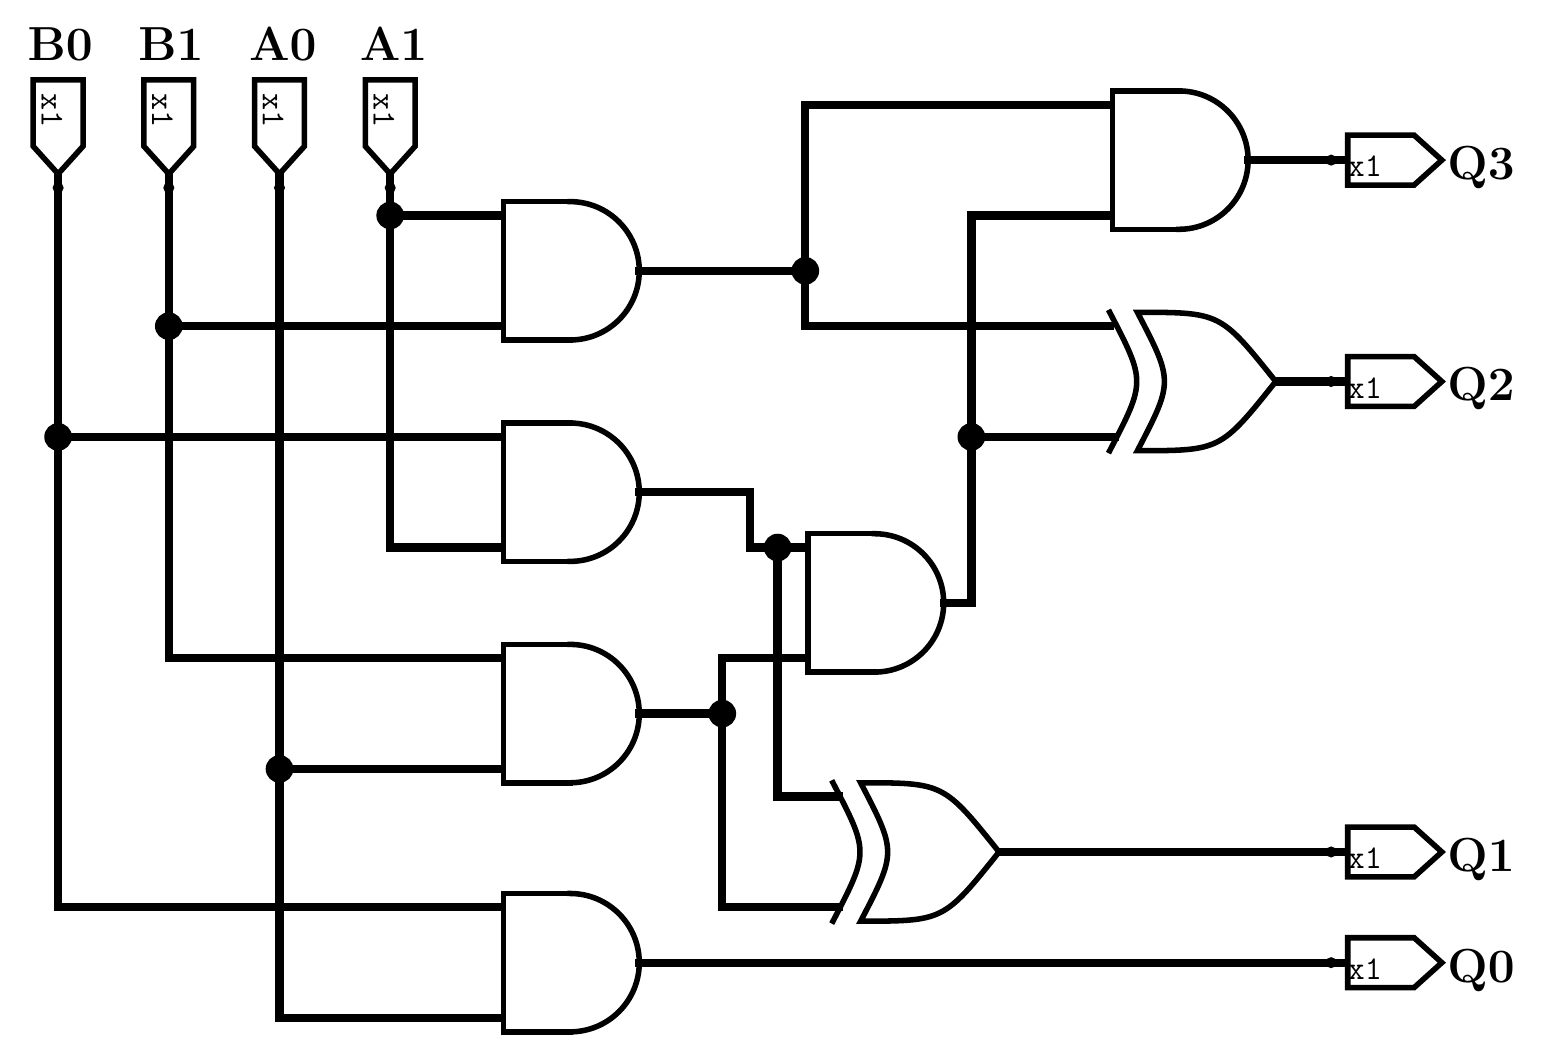
\begin{tikzpicture}[x=1pt,y=-1pt,line cap=rect]
\def\logisimfontA#1{\fontfamily{cmr}{#1}} % Replaced by logisim, original font was "SansSerif"
\def\logisimfontB#1{\fontfamily{cmtt}{#1}} % Replaced by logisim, original font was "Monospaced"
\definecolor{custcol_0_0_0}{RGB}{0, 0, 0}
\definecolor{custcol_ff_ff_ff}{RGB}{255, 255, 255}
\draw [line width=3.0pt, custcol_0_0_0 ]  (226.0,346.0) -- (476.0,346.0) ;
\draw [line width=3.0pt, custcol_0_0_0 ]  (356.0,306.0) -- (476.0,306.0) ;
\draw [line width=3.0pt, custcol_0_0_0 ]  (446.0,56.0) -- (476.0,56.0) ;
\draw [line width=3.0pt, custcol_0_0_0 ]  (226.0,256.0) -- (256.0,256.0) ;
\draw [line width=3.0pt, custcol_0_0_0 ]  (456.0,136.0) -- (476.0,136.0) ;
\draw [line width=3.0pt, custcol_0_0_0 ]  (16.0,156.0) -- (16.0,326.0) -- (176.0,326.0) ;
\draw [line width=3.0pt, custcol_0_0_0 ]  (96.0,276.0) -- (176.0,276.0) ;
\draw [line width=3.0pt, custcol_0_0_0 ]  (226.0,176.0) -- (266.0,176.0) -- (266.0,196.0) -- (276.0,196.0) ;
\draw [line width=3.0pt, custcol_0_0_0 ]  (396.0,36.0) -- (286.0,36.0) -- (286.0,96.0) ;
\draw [line width=3.0pt, custcol_0_0_0 ]  (56.0,116.0) -- (56.0,236.0) -- (176.0,236.0) ;
\draw [line width=3.0pt, custcol_0_0_0 ]  (346.0,156.0) -- (346.0,216.0) -- (336.0,216.0) ;
\draw [line width=3.0pt, custcol_0_0_0 ]  (136.0,76.0) -- (136.0,196.0) -- (176.0,196.0) ;
\fill [line width=3.0pt, custcol_0_0_0]  (256.0,256.0) ellipse (5.0 and 5.0 );
\fill [line width=3.0pt, custcol_0_0_0]  (286.0,96.0) ellipse (5.0 and 5.0 );
\fill [line width=3.0pt, custcol_0_0_0]  (346.0,156.0) ellipse (5.0 and 5.0 );
\fill [line width=3.0pt, custcol_0_0_0]  (16.0,156.0) ellipse (5.0 and 5.0 );
\fill [line width=3.0pt, custcol_0_0_0]  (276.0,196.0) ellipse (5.0 and 5.0 );
\fill [line width=3.0pt, custcol_0_0_0]  (96.0,276.0) ellipse (5.0 and 5.0 );
\fill [line width=3.0pt, custcol_0_0_0]  (56.0,116.0) ellipse (5.0 and 5.0 );
\fill [line width=3.0pt, custcol_0_0_0]  (136.0,76.0) ellipse (5.0 and 5.0 );
\draw [line width=3.0pt, custcol_0_0_0 ]  (96.0,61.0) -- (96.0,66.0) -- (96.0,276.0) -- (96.0,366.0) -- (176.0,366.0) ;
\draw [line width=2.0pt, custcol_0_0_0 ]  (87.0,51.0) -- (96.0,61.0) -- (105.0,51.0) -- (105.0,27.0) -- (87.0,27.0) -- cycle;
\logisimfontB{\fontsize{12pt}{12pt}\selectfont\node[inner sep=0, outer sep=0, custcol_0_0_0, anchor=base west, rotate=-90.0] at  (90.0,32.0)  {x1};}
\logisimfontA{\fontsize{16pt}{16pt}\fontseries{bx}\selectfont\node[inner sep=0, outer sep=0, custcol_0_0_0, anchor=base west] at  (85.0,20.0)  {A0};}
\fill [line width=2.0pt, custcol_0_0_0]  (96.0,66.0) ellipse (2.0 and 2.0 );
\draw [line width=3.0pt, custcol_0_0_0 ]  (136.0,61.0) -- (136.0,66.0) -- (136.0,76.0) -- (176.0,76.0) ;
\draw [line width=2.0pt, custcol_0_0_0 ]  (127.0,51.0) -- (136.0,61.0) -- (145.0,51.0) -- (145.0,27.0) -- (127.0,27.0) -- cycle;
\logisimfontB{\fontsize{12pt}{12pt}\selectfont\node[inner sep=0, outer sep=0, custcol_0_0_0, anchor=base west, rotate=-90.0] at  (130.0,32.0)  {x1};}
\logisimfontA{\fontsize{16pt}{16pt}\fontseries{bx}\selectfont\node[inner sep=0, outer sep=0, custcol_0_0_0, anchor=base west] at  (125.0,20.0)  {A1};}
\fill [line width=2.0pt, custcol_0_0_0]  (136.0,66.0) ellipse (2.0 and 2.0 );
\draw [line width=2.0pt, custcol_0_0_0] (201.0,121.0) arc (90.0:-90.0:25.0 and 25.0 );
\draw [line width=2.0pt, custcol_0_0_0 ]  (201.0,71.0) -- (177.0,71.0) -- (177.0,121.0) -- (201.0,121.0) ;
\draw [line width=2.0pt, custcol_0_0_0] (201.0,201.0) arc (90.0:-90.0:25.0 and 25.0 );
\draw [line width=2.0pt, custcol_0_0_0 ]  (201.0,151.0) -- (177.0,151.0) -- (177.0,201.0) -- (201.0,201.0) ;
\draw [line width=2.0pt, custcol_0_0_0] (201.0,281.0) arc (90.0:-90.0:25.0 and 25.0 );
\draw [line width=2.0pt, custcol_0_0_0 ]  (201.0,231.0) -- (177.0,231.0) -- (177.0,281.0) -- (201.0,281.0) ;
\draw [line width=2.0pt, custcol_0_0_0] (311.0,241.0) arc (90.0:-90.0:25.0 and 25.0 );
\draw [line width=2.0pt, custcol_0_0_0 ]  (311.0,191.0) -- (287.0,191.0) -- (287.0,241.0) -- (311.0,241.0) ;
\draw [line width=2.0pt, custcol_0_0_0] (421.0,81.0) arc (90.0:-90.0:25.0 and 25.0 );
\draw [line width=2.0pt, custcol_0_0_0 ]  (421.0,31.0) -- (397.0,31.0) -- (397.0,81.0) -- (421.0,81.0) ;
\draw [line width=3.0pt, custcol_0_0_0 ]  (226.0,96.0) -- (286.0,96.0) -- (286.0,116.0) -- (396.0,116.0) -- (396.0,116.0) ;
\draw [line width=3.0pt, custcol_0_0_0 ]  (396.0,76.0) -- (346.0,76.0) -- (346.0,156.0) -- (396.0,156.0) -- (398.0,156.0) ;
\draw [line width=2.0pt, custcol_0_0_0 ]  (456.0,136.0) .. controls  (436.0,111.0)  ..  (406.0,111.0) .. controls  (419.0,136.0)  ..  (406.0,161.0) .. controls  (436.0,161.0)  ..  (456.0,136.0) -- cycle ;
\draw [line width=2.0pt, custcol_0_0_0 ]  (396.0,111.0) .. controls  (409.0,136.0)  ..  (396.0,161.0) ;
\draw [line width=3.0pt, custcol_0_0_0 ]  (286.0,196.0) -- (276.0,196.0) -- (276.0,286.0) -- (296.0,286.0) -- (298.0,286.0) ;
\draw [line width=3.0pt, custcol_0_0_0 ]  (286.0,236.0) -- (256.0,236.0) -- (256.0,256.0) -- (256.0,326.0) -- (296.0,326.0) -- (298.0,326.0) ;
\draw [line width=2.0pt, custcol_0_0_0 ]  (356.0,306.0) .. controls  (336.0,281.0)  ..  (306.0,281.0) .. controls  (319.0,306.0)  ..  (306.0,331.0) .. controls  (336.0,331.0)  ..  (356.0,306.0) -- cycle ;
\draw [line width=2.0pt, custcol_0_0_0 ]  (296.0,281.0) .. controls  (309.0,306.0)  ..  (296.0,331.0) ;
\draw [line width=2.0pt, custcol_0_0_0] (201.0,371.0) arc (90.0:-90.0:25.0 and 25.0 );
\draw [line width=2.0pt, custcol_0_0_0 ]  (201.0,321.0) -- (177.0,321.0) -- (177.0,371.0) -- (201.0,371.0) ;
\draw [line width=3.0pt, custcol_0_0_0 ]  (480.0,136.0) -- (477.0,136.0) ;
\draw [line width=2.0pt, custcol_0_0_0 ]  (506.0,127.0) -- (516.0,136.0) -- (506.0,145.0) -- (482.0,145.0) -- (482.0,127.0) -- cycle;
\logisimfontB{\fontsize{12pt}{12pt}\selectfont\node[inner sep=0, outer sep=0, custcol_0_0_0, anchor=base west] at  (482.0,142.0)  {x1};}
\logisimfontA{\fontsize{16pt}{16pt}\fontseries{bx}\selectfont\node[inner sep=0, outer sep=0, custcol_0_0_0, anchor=base west] at  (518.0,143.0)  {Q2};}
\fill [line width=2.0pt, custcol_0_0_0]  (476.0,136.0) ellipse (2.0 and 2.0 );
\draw [line width=3.0pt, custcol_0_0_0 ]  (480.0,306.0) -- (477.0,306.0) ;
\draw [line width=2.0pt, custcol_0_0_0 ]  (506.0,297.0) -- (516.0,306.0) -- (506.0,315.0) -- (482.0,315.0) -- (482.0,297.0) -- cycle;
\logisimfontB{\fontsize{12pt}{12pt}\selectfont\node[inner sep=0, outer sep=0, custcol_0_0_0, anchor=base west] at  (482.0,312.0)  {x1};}
\logisimfontA{\fontsize{16pt}{16pt}\fontseries{bx}\selectfont\node[inner sep=0, outer sep=0, custcol_0_0_0, anchor=base west] at  (518.0,313.0)  {Q1};}
\fill [line width=2.0pt, custcol_0_0_0]  (476.0,306.0) ellipse (2.0 and 2.0 );
\draw [line width=3.0pt, custcol_0_0_0 ]  (480.0,346.0) -- (477.0,346.0) ;
\draw [line width=2.0pt, custcol_0_0_0 ]  (506.0,337.0) -- (516.0,346.0) -- (506.0,355.0) -- (482.0,355.0) -- (482.0,337.0) -- cycle;
\logisimfontB{\fontsize{12pt}{12pt}\selectfont\node[inner sep=0, outer sep=0, custcol_0_0_0, anchor=base west] at  (482.0,352.0)  {x1};}
\logisimfontA{\fontsize{16pt}{16pt}\fontseries{bx}\selectfont\node[inner sep=0, outer sep=0, custcol_0_0_0, anchor=base west] at  (518.0,353.0)  {Q0};}
\fill [line width=2.0pt, custcol_0_0_0]  (476.0,346.0) ellipse (2.0 and 2.0 );
\draw [line width=3.0pt, custcol_0_0_0 ]  (480.0,56.0) -- (477.0,56.0) ;
\draw [line width=2.0pt, custcol_0_0_0 ]  (506.0,47.0) -- (516.0,56.0) -- (506.0,65.0) -- (482.0,65.0) -- (482.0,47.0) -- cycle;
\logisimfontB{\fontsize{12pt}{12pt}\selectfont\node[inner sep=0, outer sep=0, custcol_0_0_0, anchor=base west] at  (482.0,62.0)  {x1};}
\logisimfontA{\fontsize{16pt}{16pt}\fontseries{bx}\selectfont\node[inner sep=0, outer sep=0, custcol_0_0_0, anchor=base west] at  (518.0,63.0)  {Q3};}
\fill [line width=2.0pt, custcol_0_0_0]  (476.0,56.0) ellipse (2.0 and 2.0 );
\draw [line width=3.0pt, custcol_0_0_0 ]  (56.0,61.0) -- (56.0,66.0) -- (56.0,116.0) -- (176.0,116.0) ;
\draw [line width=2.0pt, custcol_0_0_0 ]  (47.0,51.0) -- (56.0,61.0) -- (65.0,51.0) -- (65.0,27.0) -- (47.0,27.0) -- cycle;
\logisimfontB{\fontsize{12pt}{12pt}\selectfont\node[inner sep=0, outer sep=0, custcol_0_0_0, anchor=base west, rotate=-90.0] at  (50.0,32.0)  {x1};}
\logisimfontA{\fontsize{16pt}{16pt}\fontseries{bx}\selectfont\node[inner sep=0, outer sep=0, custcol_0_0_0, anchor=base west] at  (45.0,20.0)  {B1};}
\fill [line width=2.0pt, custcol_0_0_0]  (56.0,66.0) ellipse (2.0 and 2.0 );
\draw [line width=3.0pt, custcol_0_0_0 ]  (16.0,61.0) -- (16.0,66.0) -- (16.0,156.0) -- (176.0,156.0) ;
\draw [line width=2.0pt, custcol_0_0_0 ]  (7.0,51.0) -- (16.0,61.0) -- (25.0,51.0) -- (25.0,27.0) -- (7.0,27.0) -- cycle;
\logisimfontB{\fontsize{12pt}{12pt}\selectfont\node[inner sep=0, outer sep=0, custcol_0_0_0, anchor=base west, rotate=-90.0] at  (10.0,32.0)  {x1};}
\logisimfontA{\fontsize{16pt}{16pt}\fontseries{bx}\selectfont\node[inner sep=0, outer sep=0, custcol_0_0_0, anchor=base west] at  (5.0,20.0)  {B0};}
\fill [line width=2.0pt, custcol_0_0_0]  (16.0,66.0) ellipse (2.0 and 2.0 );
\end{tikzpicture}

